\documentclass[10pt,twocolumn,letterpaper]{article}

\usepackage{cvpr}
\usepackage{times}
\usepackage{epsfig}
\usepackage{graphicx}
\usepackage{amsmath}
\usepackage{amssymb}
\usepackage{float}

% Include other packages here, before hyperref.

% If you comment hyperref and then uncomment it, you should delete
% egpaper.aux before re-running latex.  (Or just hit 'q' on the first latex
% run, let it finish, and you should be clear).
\usepackage[breaklinks=true,bookmarks=false]{hyperref}

\cvprfinalcopy % *** Uncomment this line for the final submission

\def\cvprPaperID{****} % *** Enter the CVPR Paper ID here
\def\httilde{\mbox{\tt\raisebox{-.5ex}{\symbol{126}}}}

% Pages are numbered in submission mode, and unnumbered in camera-ready
%\ifcvprfinal\pagestyle{empty}\fi
\setcounter{page}{1}
\begin{document}

%%%%%%%%% TITLE
\title{Improving Parametric Colorization Methods Using Discriminators }

\author{Emily Mu\\
Massachusetts Institute of Technology\\
6.869\\
{\tt\small emilymu@mit.edu}
% For a paper whose authors are all at the same institution,
% omit the following lines up until the closing ``}''.
% Additional authors and addresses can be added with ``\and'',
% just like the second author.
% To save space, use either the email address or home page, not both
\and
Ka Wai Lee\\
Massachusetts Institute of Technology\\
6.869\\
{\tt\small kwlee@mit.edu}
}

\maketitle
%\thispagestyle{empty}

%%%%%%%%% ABSTRACT
\begin{abstract}
We utilize a discriminator trained on top of a state-of-the-art colorization generator to improve plausible colorization of specifically difficult grayscale inputs. Determining a plausible colored version of a grayscale photograph is inherently an underconstrained problem so early data-driven attempts at producing plausible colored often resulted in undersaturated non-realistic images. Current state-of-the-art approaches are trained on millions of colored examples and incorporate intermediate steps and tailored loss functions to mediate undersaturation. Inspired by the success of generative adversarial networks on image-to-image translation problems, we built a discriminator on the results of a state-of-the-art colorizer to demonstrate the improvements that can still be made in this field. We demonstrate that discriminators can still determine the difference between computer-generated and actual colored photographs with a high-degree of accuracy, picking up on the same color confusions and inconsistencies that human users do. We then use the results of our discriminator to fine-tune the original generator to produce more vibrant and plausible colorizations for failure cases. 
\end{abstract}

%%%%%%%%% BODY TEXT
\section{Introduction}

Coloring a grayscale image in a vivid and realistic way is simple for the human imagination (Figure 1). However, the range of realistic colorizations can be very difficult to determine since many possibilities exist and a third of the information has been lost. Our imagination fills in some of this information with previous experience, we know logically that grass tends to be green and the sky tends to be blue. Much progress has been made already in generating photo-realistic images [5. 9]. In fact, the colorization task has been found to be a competitive method for self-supervised representation learning [3]. 

\begin{figure}[htp]

\centering
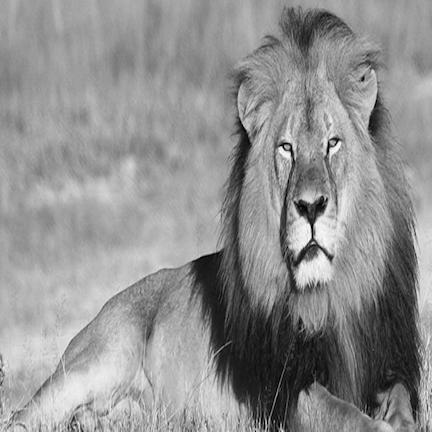
\includegraphics[width=.1\textwidth]{ex_1_bw.jpg} 
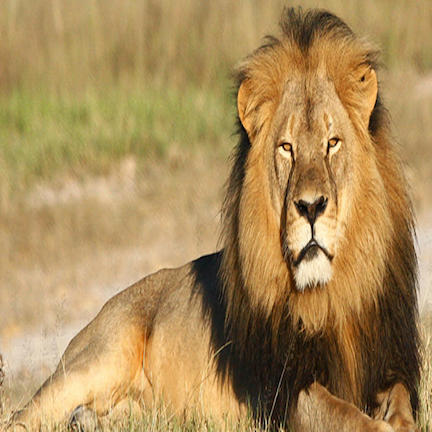
\includegraphics[width=.1\textwidth]{ex_1.jpg}
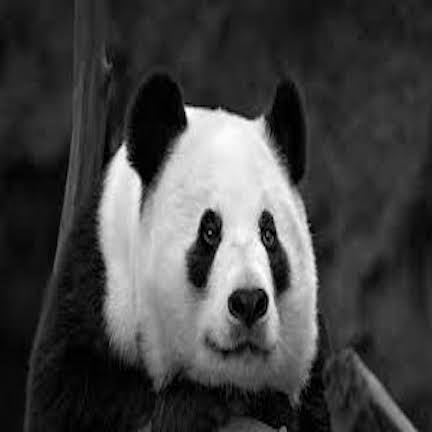
\includegraphics[width=.1\textwidth]{ex_2_bw.jpg} 
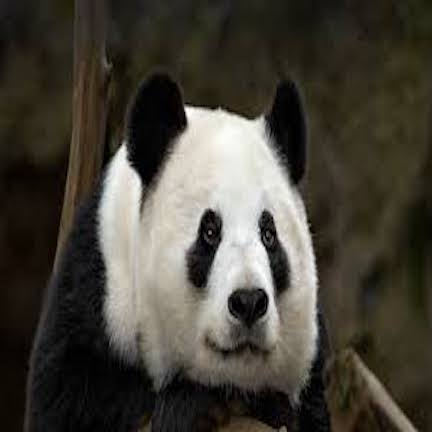
\includegraphics[width=.1\textwidth]{ex_2.jpeg} \\
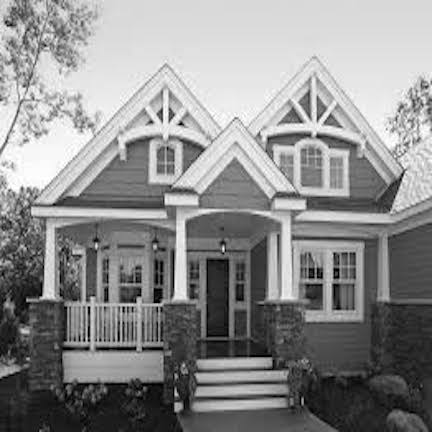
\includegraphics[width=.1\textwidth]{ex_3_bw.jpg} 
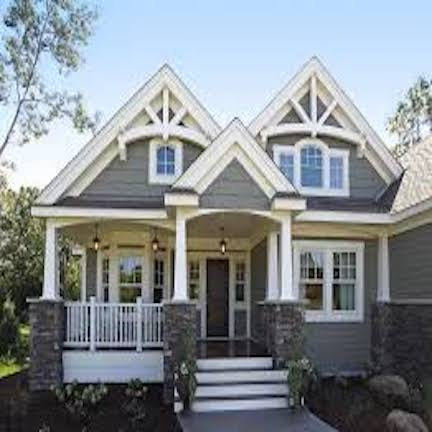
\includegraphics[width=.1\textwidth]{ex_3.jpeg}
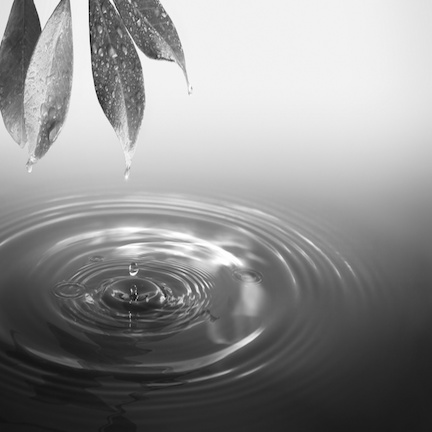
\includegraphics[width=.1\textwidth]{ex_4_bw.jpg}
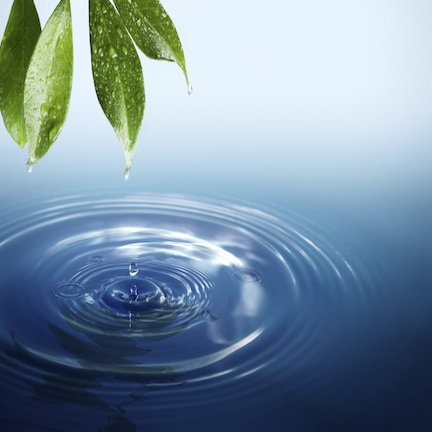
\includegraphics[width=.1\textwidth]{ex_4.jpg} \\
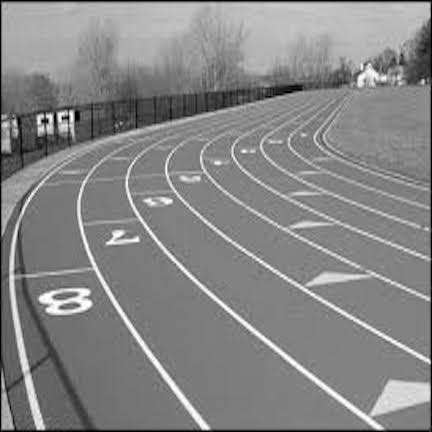
\includegraphics[width=.1\textwidth]{ex_5_bw.jpg} 
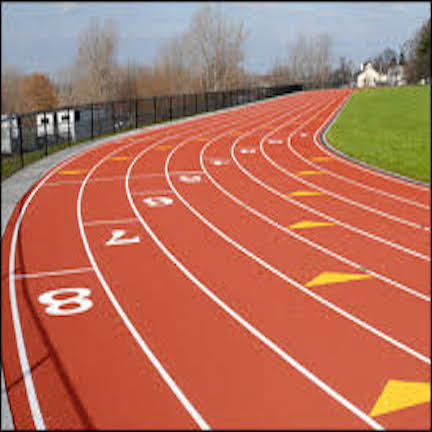
\includegraphics[width=.1\textwidth]{ex_5.jpeg}
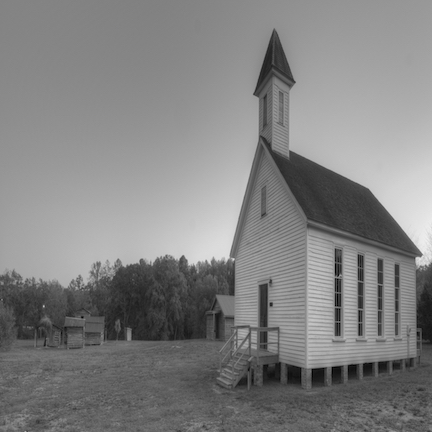
\includegraphics[width=.1\textwidth]{ex_6_bw.jpg} 
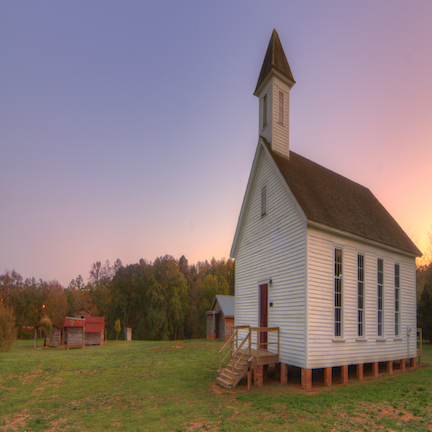
\includegraphics[width=.1\textwidth]{ex_6.jpg}
\caption{Some examples of grayscale and ground-truth colored corresponding input/output pairs}

\end{figure}

Current methods of evaluating synthesized images include testing human observers by asking observers to distinguish computer generated and photo-realistic images. Human observers are presented with the ground truth colorization and the synthesized colorization and asked to identify the fake image. Current state-of-the-art colorizers are able to fool participants over $30\%$ of the time, with $50\%$ being equivalent to ground truth colorization [5, 8]. Some of these high-performing colorizer architectures will be discussed in related work, but it is important to note that many of these incorporate loss functions specifically to reduce saturation loss [1,2,5,9]. 

Relatedly, conditional adversarial networks (cGANs) have been shown to be flexible general-purpose solutions for image-to-image translation problems [4,8]. These translation problems are defined by translating one image representation to another and colorization is such and example. Conditional adversarial networks consist of training a generative model and a discriminator concurrently. The discriminator attempts to determine if the output of the generator model is real or fake. Consequently, cGANs have been shown to be able to learn a loss function that adapts automatically to the data and perform well on many image-to-image translation problems. By the same method of evaluation described above, a cGAN trained with additional L1 loss was able to fool observers $22.5\%$ of the time.

Although cGANs have been shown to work well on image-to-image translation problems, state-of-the-art colorizers do not train with cGAN loss. Rather, they tend to define specific loss functions for more traditional convolutional neural networks to reduce saturation loss. In this paper, we explore training a discriminator on top of the results of the best generators to look at how to improve existing colorizers. We had a two-fold goal for this project: (1) to understand and (2) to improve failure cases for existing state-of-the-art colorizers. We used the generator designed by Zhang et al. for this project. After training a discriminator on ground truth and images generated by the algorithm, we find that the discriminator can determine the difference between fake and real images with an error of only $2.8\%$. We examine these error cases and the results of the discriminator to demonstrate that the discriminator can find the similar differences between fake and real images that human perception can, including ambiguous coloration, inaccurate long-range consistency, and unnatural tones [6, 7]. We then utilize our discriminator to identify and fine-tune the existing generator for the most difficult failure cases and demonstrate that we can construct more feasible colorizations for these cases (footnote: code).

Our contributions in this paper are as follows: to allow for better understanding of areas for improvement in image colorization, to provide a framework to automatically identify and tackle failure cases of existing generators, and to demonstrate the success of this framework to improve these cases. 

\subsection{Related Work}

Colorization algorithms usually take one of two forms: non-parametric and parametric. Non-parametric models tend to use user-guided inputs or references from scribbles to determine accurate image colorization [5, 9]. Parametric models utilize large datasets by learning how to predict color as either a continuous or quantized output and tend to be more self-supervised or automatic [2]. This paper will be focused of improving this second class of parametric models.

We define state-of-the-art parametric colorizers as methods that fool observers with over $30\%$ reported accuracy, as defined in the introduction. Several recently developed architectures exist in this category. One method developed by Zhang et. al poses the colorization problem as a classification tast and used class-rebalancing at training time to capture a wider variety of colors. Concurrently, a method developed by Larsson et al. uses a modified VGG network to predict per-pixel histograms. Iizuka et al. also developed a similarly well-performing method by using a two-stream architecture to capture both local and global features of the image.

Conditional adversarial networks (cGANs) have been shown to work well for general image-to-image translation problems, achieving a $22.5\%$ accuracy on the colorization problem. Traditional cGANs train a generator (conditioned on some input) and a discriminator concurrently with the generator attempting to minimize discriminator accuracy on real and fake data. Inspired by the cGAN architecture, we train a discriminator on top of an already tuned parametric generator in order to evaluation generation results and learn how to improve training. 

We selected Zhang et al as the example generator for improvement because the source code and examples are open source and well documented. Comparisons made in the Zhang et al paper show that the results of their method are comparable to the other methods described [9]. Furthermore, their method is hosted on Algorithmia, allowing for easy data generation and testing. The specifics of their generator model will be described in the next section.

\section{Approach}

We train a CNN to classify generated and ground-truth colored imaged using the architecture shown in Figure 2. In this section, we discuss the open source architecture of the generator designed and implemented by Zhang et al. and the architecture of the discriminator we implemented which can be found on our public repository.

\subsection{Generator Architecture}

\begin{figure*}[htp]

\centering
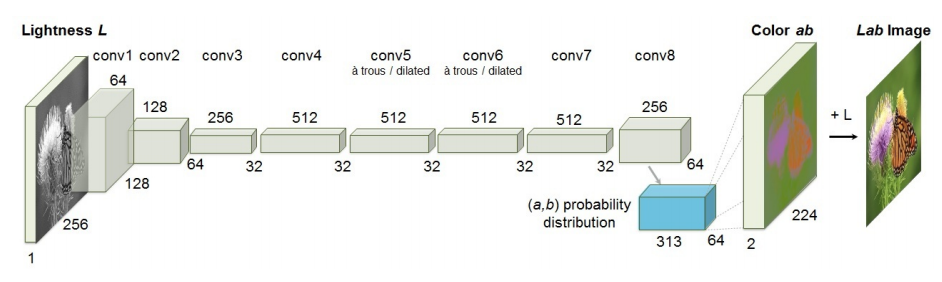
\includegraphics[width= \textwidth]{gen_arch.png} 
\caption{The generator architecture designed by Zhang et al. Each conv layer consists of 2 or 3 repeated conv and ReLU layers followed by a BatchNorm layer. Changes in resolution are through down and upsampling.}

\end{figure*}

The generator method was designed by Zhang et al., and we provide a brief description of method here. Further analysis of their method and its performance can be found in their paper. Given an input grayscale image, one potential method trains a CNN to map that image input channel $X$ to two associated color channels $\hat{Y} = F(X)$. The most natural loss function for CNNs is the Euclidean loss function between ground truth and predicted values:

$$L_2(\hat{Y}, Y) = \frac{1}{2} \sum_{h,w} ||Y_{h,w} - \hat{Y}_{h,w}||_2^2$$

The problem with just using this loss function, however, is that the optimal solution is a mean of all plausible values, which results in grayish, unsaturated images. Consequently, to improve this, the problem is treated as a classification instead, where the input is mapped to a distribution over the quantized $ab$ color space. Instead of learning $\hat{Y}$, we learn $\hat{Z} = G(X)$ where $\hat{Z}$ is a probability distribution over possible colors. We can then convert our ground truth color $Y$ to a vector $Z$ by function $Z = H_{gt}^{-1}(Y)$, using a soft-encoding scheme. Given this definition of $Z$, we can now use multinomial cross entropy loss to define our new loss function

$$L_{cl}(\hat{Z}, Z) =  - \sum_{h,w}v(Z_{h,w})\sum_q Z_{h,w,q} \log{\hat{Z}_{h,w,q}}$$

$v$ is a weight that allows for the rebalancing of the loss baes on color-class during training. This is necessary because natural images tend towards desaturated or low $ab$ values which dominate the loss function. Thus, in order to prevent this, we weight the loss of each pixel based on color rarity, analogous to resampling the training space. We define function $v$ as follows in terms of its closest $ab$ bin $q*$.

$$v(Z_{h,w}) = w_{q*}, \text{where } q* = arg max_q Z_{h,w,q}$$

In order to estimate the weighting factor $w$, we take the smoothed distribution of colors and weight it weight it with a uniform distribution. We then make the weighting factor inversely related to this new distribution. We then normalize so that the expected value of the weighting factor is 1. The specific experiments to calculate and determine this weighting can be found in the original paper. 

Finally, we must compute the function $H$ that maps the color distribution $\hat{Z}$ to a single estimate in $ab$ space $\hat{Y}$. Taking the mean has a similar problem to using the Euclidean loss--results tend to be desaturated. However, taking the mode of the distribution for each pixel also results in very splotchly, spatially inconsistent results. Thus, we compute a combination anneal-mean of the distribution as follows

$$H(Z_{h,w}) = \mathbb{E}[f_T(Z_{h,w})], f_T(z) = \frac{\text{exp}(\text{log}(z)/T)}{\sum_q\text{exp}(\text{log}(z)/T)}$$

Experiments with annealed mean demonstrated that a temperature of $T = 0.38$ worked well for this function. The final system composes the CNN $G$ with this annealed-mean operation $H$ to construct a final determined image output. 

\subsection{Discriminator Architecture}

\begin{figure*}[htp]

\centering
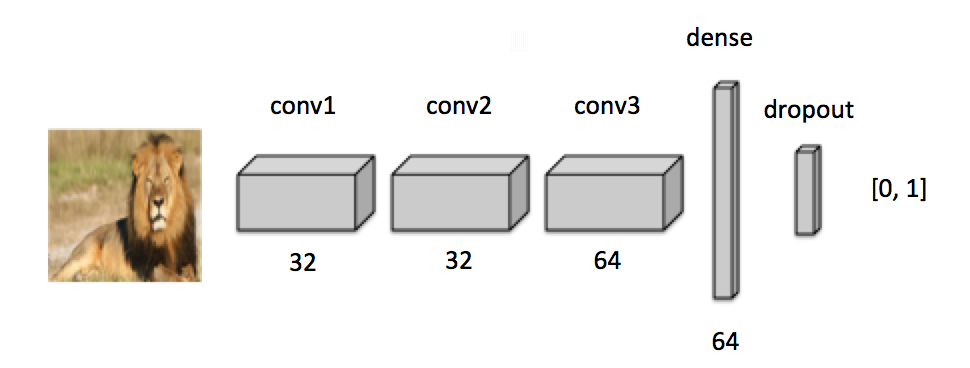
\includegraphics[width= \textwidth]{disc_arch.png} 
\caption{The discriminator architecture is shown here. The three-channel image is passed through three convolutional layers with $3 \times 3$ filters. Each convolutional layer is followed by ReLU activation and a $2 \times 2$ max pooling layer. This output is then flattened and passed through a fully connected layer of size 64 with ReLU. Dropout is then added and a sigmoid output of a single unit converts the output to a value from the range of 0 to 1.}

\end{figure*}

We trained a discriminator on the results of the generator and the ground truth colors of input images. These fake and real images were first formatted to have width and height of 150 pixels and normalized.

These normalized images were then passed through two convolutional layers with 32 hidden units and filter size of 3. Each convolutional layer is followed by a ReLU activation and a $2 \times 2$ max pooling layer. This output is then passed through a third convolutional layer with 64 hidden units and a filter size of 3. Again ReLU activation and $2 \times 2$ max pooling layer. This output is then flattened and passed through a fully connected layer of size 64 with ReLU activation. Dropout is added to prevent overfitting and then a sigmoid output of a single unit is computed to determine classification. Figure 3 is a visual representation of this architecture.

The model is trained with binary cross-entropy loss 

$$L = - \sum_i y_i' \log_2{y_i}$$

where $y_i'$ represents the predicted label and $y_i$ represents the actual label. The learning rates are updated with the RMSprop optimizer developed by Geoffrey Hinton.

\section{Results}

In this section, we describe the results of training our discriminator, including discriminator performance and our qualitative observations. We then discuss how we use the results of the discriminator to fine-tune performance of the generator on failure cases. 

\subsection{Training the discriminator}

We use the same 20000 images (10000 generated and 10000 corresponding ground truth) that were used to test participants in the study by Zhang et al. to train our discriminator. These images are a subsampling of the ImageNet dataset. We separate out the 20000 examples into a 16000 image training set (8000 corresponding pairs of generated and ground truth images) and 4000 image validation set (2000 corresponding pairs of generated and ground truth images). We trained in batches of size 16 and we found that validation accuracy plateaued at around 10 epochs. The training and validation accuracy over epochs is plotted in Figure 4. 

\begin{figure}[htp]

\centering
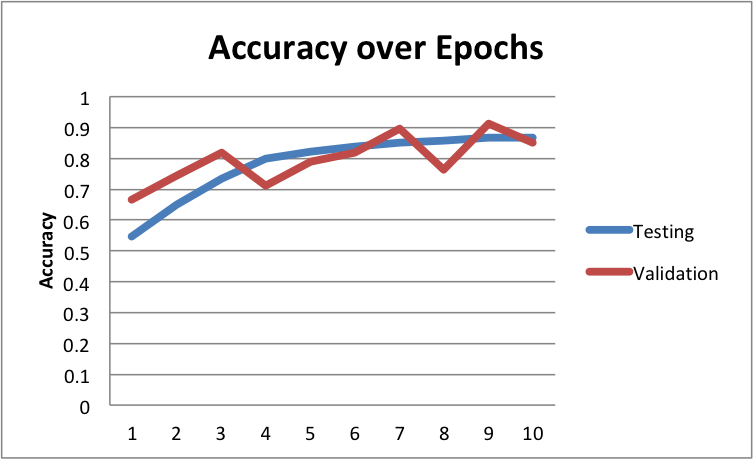
\includegraphics[width= 0.45 \textwidth]{training.png} 
\caption{The training and validation accuracy over 10 epochs. Note that accuracy plateaus around $86\%$ for both training and validation data sets.}

\end{figure}

\subsection{Discriminator Performance}

In order to compare our discriminator performance to human performance, we compared the resulting value for each of the images in each corresponding fake and real colorization for the validation dataset. We then determined which resulting value was higher in order to determine which image the discriminator would predict to be "ground truth". We found only 58 examples out of 2000 image pairs that the discriminator would predict the computer generated image over the actual ground truth image as ground truth. Note that this means that by the same ground truth versus colorization test, our discriminator is fooled $2.8\%$ of the time in comparison to $32\%$ when presented to human observers as described in the paper by Zhang et al [9]. 

\begin{table}
\begin{center}
\begin{tabular}[H]{|l|c|}
\hline
Testing & Labeled Real \\
\hline \hline
Humans (AMT) & 32.3 $\%$ \\
Discriminator & 2.8 $\%$ \\
\hline
\end{tabular}
\end{center}
\caption{Our discriminator labeled computer generated images as real $2.8\%$ of the time in comparison to humans on Amazon Turk who labeled computer generated images as real $32.3\%$ of the time.}
\end{table}

\subsection{Qualitative Observations}

In order to better understand how our discriminator is classifying computer generated vs ground truth images, we look at some examples of what the discriminator considers to be the most computer generated and most real images. Ten of the images that the discriminator considers the most computer generated and their corresponding ground truth images are presented in Figure 5. Similarly, ten of the images that the discriminator considers the most real and their corresponding computer generated images are presented in Figure 6. Some of the 58 incorrectly classified images are displayed in Figure 7. 

\begin{figure}[htp]

\centering
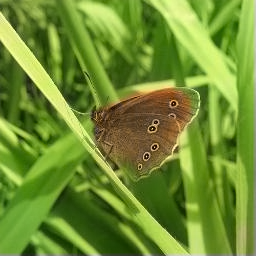
\includegraphics[width=.10\textwidth]{analysis/most_cr_imgs_tot/48000.png} 
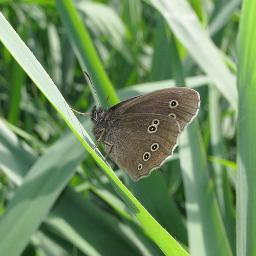
\includegraphics[width=.10\textwidth]{analysis/most_cr_imgs_tot/gt/48000.png} 
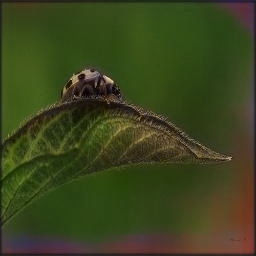
\includegraphics[width=.10\textwidth]{analysis/most_cr_imgs_tot/48057.png} 
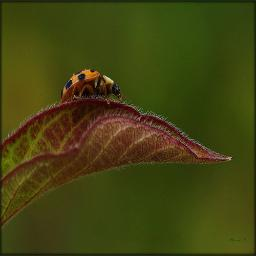
\includegraphics[width=.10\textwidth]{analysis/most_cr_imgs_tot/gt/48057.png} \\
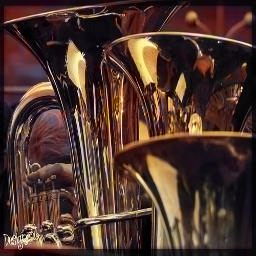
\includegraphics[width=.10\textwidth]{analysis/most_cr_imgs_tot/48506.png} 
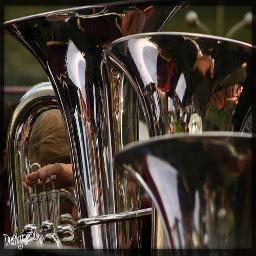
\includegraphics[width=.10\textwidth]{analysis/most_cr_imgs_tot/gt/48506.png} 
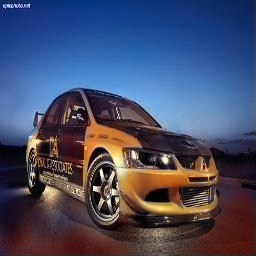
\includegraphics[width=.10\textwidth]{analysis/most_cr_imgs_tot/48515.png} 
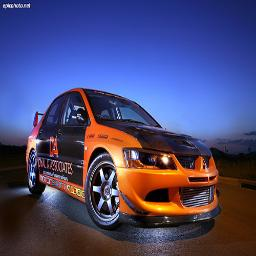
\includegraphics[width=.10\textwidth]{analysis/most_cr_imgs_tot/gt/48515.png}  \\
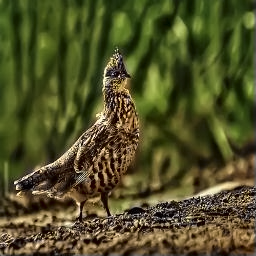
\includegraphics[width=.10\textwidth]{analysis/most_cr_imgs_tot/48600.png} 
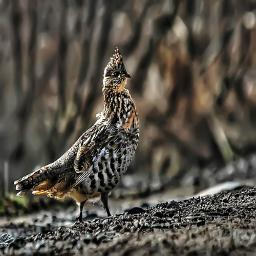
\includegraphics[width=.10\textwidth]{analysis/most_cr_imgs_tot/gt/48600.png} 
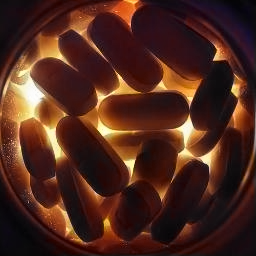
\includegraphics[width=.10\textwidth]{analysis/most_cr_imgs_tot/48929.png} 
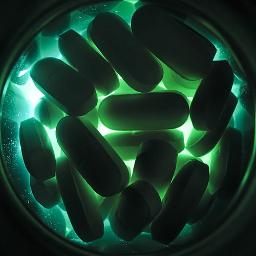
\includegraphics[width=.10\textwidth]{analysis/most_cr_imgs_tot/gt/48929.png}  \\
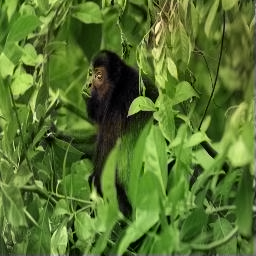
\includegraphics[width=.10\textwidth]{analysis/most_cr_imgs_tot/48931.png} 
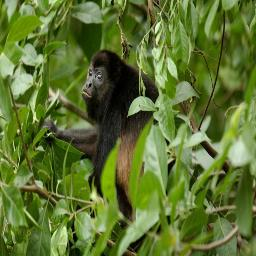
\includegraphics[width=.10\textwidth]{analysis/most_cr_imgs_tot/gt/48931.png} 
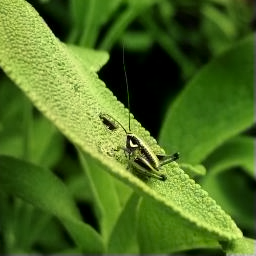
\includegraphics[width=.10\textwidth]{analysis/most_cr_imgs_tot/49637.png} 
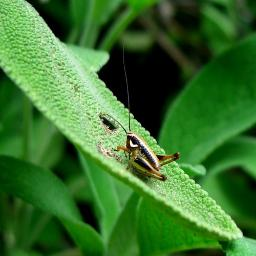
\includegraphics[width=.10\textwidth]{analysis/most_cr_imgs_tot/gt/49637.png}  \\
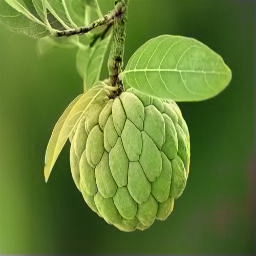
\includegraphics[width=.10\textwidth]{analysis/most_cr_imgs_tot/49676.png} 
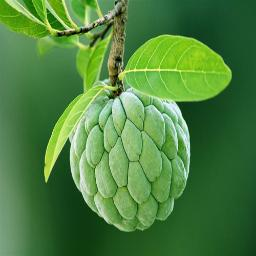
\includegraphics[width=.10\textwidth]{analysis/most_cr_imgs_tot/gt/49676.png} 
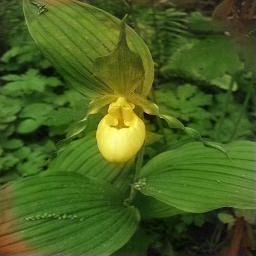
\includegraphics[width=.10\textwidth]{analysis/most_cr_imgs_tot/49905.png} 
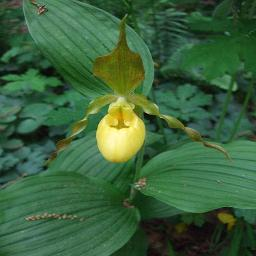
\includegraphics[width=.10\textwidth]{analysis/most_cr_imgs_tot/gt/49905.png}  \\
\caption{The 10 images the discriminator considers the most computer generated are located on the left of each pair. The corresponding ground truth image is located on the right.}

\end{figure}

\begin{figure}[htp]

\centering
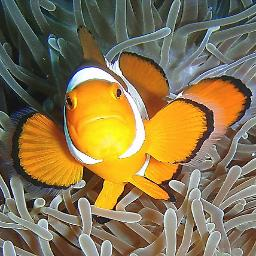
\includegraphics[width=.10\textwidth]{analysis/most_gt_imgs_tot/49442.png} 
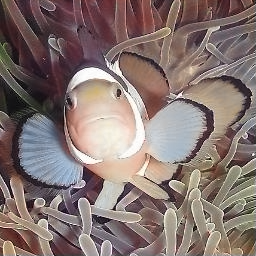
\includegraphics[width=.10\textwidth]{analysis/most_gt_imgs_tot/cr/49442.png} 
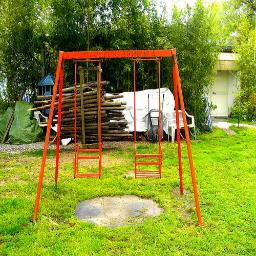
\includegraphics[width=.10\textwidth]{analysis/most_gt_imgs_tot/49444.png} 
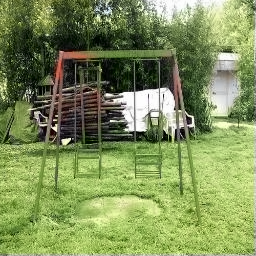
\includegraphics[width=.10\textwidth]{analysis/most_gt_imgs_tot/cr/49444.png} \\
\includegraphics[width=.10\textwidth]{analysis/most_gt_imgs_tot/49455.png} 
\includegraphics[width=.10\textwidth]{analysis/most_gt_imgs_tot/cr/49455.png} 
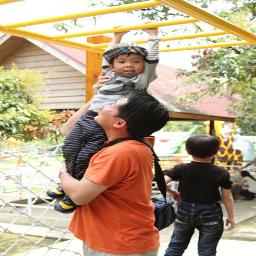
\includegraphics[width=.10\textwidth]{analysis/most_gt_imgs_tot/49467.png} 
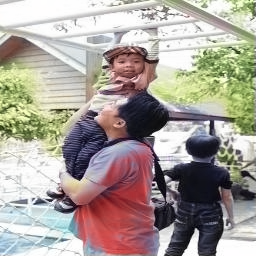
\includegraphics[width=.10\textwidth]{analysis/most_gt_imgs_tot/cr/49467.png}  \\
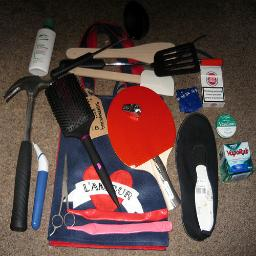
\includegraphics[width=.10\textwidth]{analysis/most_gt_imgs_tot/49490.png} 
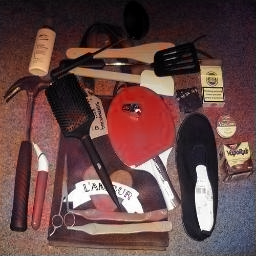
\includegraphics[width=.10\textwidth]{analysis/most_gt_imgs_tot/cr/49490.png} 
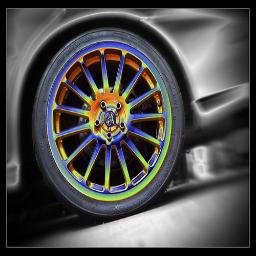
\includegraphics[width=.10\textwidth]{analysis/most_gt_imgs_tot/49493.png} 
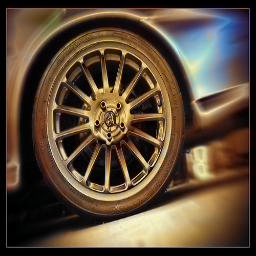
\includegraphics[width=.10\textwidth]{analysis/most_gt_imgs_tot/cr/49493.png}  \\
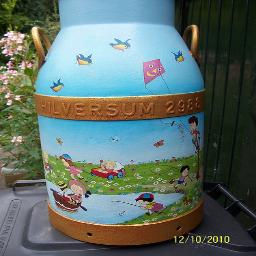
\includegraphics[width=.10\textwidth]{analysis/most_gt_imgs_tot/49505.png} 
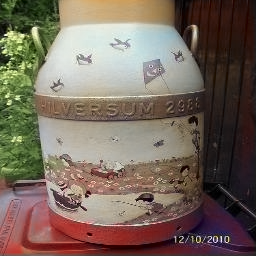
\includegraphics[width=.10\textwidth]{analysis/most_gt_imgs_tot/cr/49505.png} 
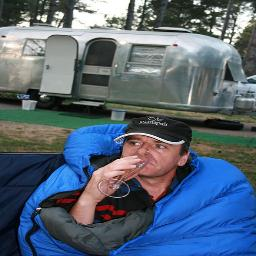
\includegraphics[width=.10\textwidth]{analysis/most_gt_imgs_tot/49508.png} 
\includegraphics[width=.10\textwidth]{analysis/most_gt_imgs_tot/cr/49508.png}  \\
\includegraphics[width=.10\textwidth]{analysis/most_gt_imgs_tot/49519.png} 
\includegraphics[width=.10\textwidth]{analysis/most_gt_imgs_tot/cr/49519.png} 
\includegraphics[width=.10\textwidth]{analysis/most_gt_imgs_tot/49538.png} 
\includegraphics[width=.10\textwidth]{analysis/most_gt_imgs_tot/cr/49538.png}  \\
\caption{The 10 images the discriminator considers the most real are located on the left of each pair. The corresponding computer generated image is located on the right.}

\end{figure}

\begin{figure}[htp]

\centering
\includegraphics[width=.10\textwidth]{analysis/incorrect_classification/cr/48016.png} 
\includegraphics[width=.10\textwidth]{analysis/incorrect_classification/gt/48016.png} 
\includegraphics[width=.10\textwidth]{analysis/incorrect_classification/cr/48030.png} 
\includegraphics[width=.10\textwidth]{analysis/incorrect_classification/gt/48030.png} \\
\includegraphics[width=.10\textwidth]{analysis/incorrect_classification/cr/48272.png} 
\includegraphics[width=.10\textwidth]{analysis/incorrect_classification/gt/48272.png} 
\includegraphics[width=.10\textwidth]{analysis/incorrect_classification/cr/48280.png} 
\includegraphics[width=.10\textwidth]{analysis/incorrect_classification/gt/48280.png} \\
\includegraphics[width=.10\textwidth]{analysis/incorrect_classification/cr/48464.png} 
\includegraphics[width=.10\textwidth]{analysis/incorrect_classification/gt/48464.png} 
\includegraphics[width=.10\textwidth]{analysis/incorrect_classification/cr/48556.png} 
\includegraphics[width=.10\textwidth]{analysis/incorrect_classification/gt/48556.png}  \\
\includegraphics[width=.10\textwidth]{analysis/incorrect_classification/cr/48563.png} 
\includegraphics[width=.10\textwidth]{analysis/incorrect_classification/gt/48563.png} 
\includegraphics[width=.10\textwidth]{analysis/incorrect_classification/cr/48567.png} 
\includegraphics[width=.10\textwidth]{analysis/incorrect_classification/gt/48567.png}  \\
\includegraphics[width=.10\textwidth]{analysis/incorrect_classification/cr/49338.png} 
\includegraphics[width=.10\textwidth]{analysis/incorrect_classification/gt/49338.png} 
\includegraphics[width=.10\textwidth]{analysis/incorrect_classification/cr/49479.png} 
\includegraphics[width=.10\textwidth]{analysis/incorrect_classification/gt/49479.png}   \\
\caption{A sampling of 10 of the 58 pairs of images that the discriminator incorrectly identifies as real. The computer generated image appears on the left and the corresponding real image appears on the right.}

\end{figure}


Referring to the images, we see that the most computer-generated images have many issues previously identified in computer generated colorization. These examples fail to capture long-range consistencies in the image, often resulting in strange red patches in the image. These images also tend to have a strange unnatural sepia tone.

Notice that the most ground truth images often have a variety of bright colors and tend to be vibrant with patterns. The corresponding computer generated images have a difficult time capturing the details and saturation of the images. 

Both of these sets of images help demonstrate that the discriminator is also picking up on some of the details that human perception does to discriminate between computer generated and real images. This can further be demonstrated in Figure 7, which contains a sampling of the 58 images that are incorrectly classified by the discriminator. Notice that the computer generated image sometimes produces more realistic colorations than the real images and the real images seem unsaturated or dull in comparison. 

\subsection{Fine-Tuning the Generator}

We use the difficult real images to fine-tune the generator to improve performance on these failure cases. In order to do this, we determine the 2000 most ground truth images from the classifier. Note that all of these images are originally ground truth images as well. We then split these into a training set of 1600 images and a test set of 400 images randomly. Beginning with the parameters of the original generator, we train with these 1600 images to produce a new set of parameters. This new tuned model is then run on the test set. A sampling of the test set with ground truth, original colorization, and new fined-tuned colorization is shown in Figure 8. Notice that our new fine-tuned colorization helps preserve long-range consistencies and help retain image vibrancy better than the original generator. 

Note that we attempted to prevent overfitting by dividing into a training and testing set and attempting trials on our own images but that overfitting to these problem cases may still be occurring. Future work may include identifying best generators for different image types. 

\section{Conclusion and Future Work}

Evaluating and colorizing images is a difficult task because it is under-constrained. In this paper, we built a discriminator to allow for better understanding of areas for improvement in image colorization and to provide a framework to automatically identify and tackle failure cases of existing generators, and we used this framework to retrain the generator to improve on these cases. 

Several directions for future work exist to improve image classification. One potential method to improve state-of-the-art networks may be to include a discriminator while training the generator and minimizing a cGAN loss combined with the original loss functions. Another method may be to train a discriminator and use the discriminator to automatically identify and improve failure cases. 

\section{Acknowledgements}

The authors would like to thank Professor Freeman and Professor Torralba for teaching this course and the rest of the 6.869 course staff for all their help in understanding the material and for the inspiration and review of this project.

\section{Contribution}

I (Emily) believe that we split work evenly on this project. We both came up with the original idea and discuss project plans. I created and trained the original discriminator and Joanne trained the generator on our difficult images. We analyzed the results of the discriminator and generator together and we split the writing and editing of this paper. We also worked on and practiced the presentation together.

\begin{thebibliography}{1}

  \bibitem{notes} Charpiat, G., Hofmann, M., Sch$\ddot{o}$lkopf, B.: Automatic image colorization via multimodal predictions. In: Computer Vision-ECCV 2008. Springer (2008) 126-139
 \bibitem{notes} Cheng, Z. Yang, Q., Sheng, B.: Deep colorization. In: Proceedings of the IEEE International Conference on Computer Vision. (2016) 415-423
 \bibitem{notes} Donahue, J., Kra$\ddot{a}$henb$\ddot{u}$hl, P., Darrell, T.: Adversarial feature learning. arXiv prepreing arXiv:1605.09782 (2016)
 \bibitem{notes} Isola, P., Zhu, J., Zhou, T., Efros, A.,: Image-to-Image Translation with Conditional Adversarial Networks. In: CoRR (2016)
  \bibitem{notes} Larsson, G., Maire, M., Shakhnarovich, G.: Learning representations for automatic colorization. In: ECCV (2016)
 \bibitem{notes} Ramanarayanan, G., Ferwerda, J., Walter, B., Bala, K.: Visual equivalence: towards a new standard for image fidelity. ACM Transactions on Graphics (TOG) \textbf{26} (3) (2007) 76
 \bibitem{notes} Russakovsky, O., Deng, J., Su, H., Krause, J., Satheesh, S., Ma, S., Huang, Z., Karpathy, A., Khosla, A., Bernstein, M., Berg, A.C., Fei-Fei, L.: ImageNet Large Scale Visual Recognition Challenge. International Journal of Computer Vision (IJCV) 115(3) (2015)
  \bibitem{notes} X. Wang and A. Gupta. Generative image modeling using style and structure adversarial networks. In: ECCV (2016)
 \bibitem{notes} Zhang, R., Isola, P., Efros, A.A.: Colorful image colorization. In: ECCV (2016)


 \end{thebibliography}

\end{document}
